\documentclass[conference]{IEEEtran}

\usepackage[T1]{fontenc}
\usepackage[utf8]{inputenc}
\usepackage{amsmath}
\usepackage{booktabs}
\usepackage{cite}
\usepackage{graphicx}
\usepackage[hidelinks]{hyperref}
\graphicspath{{figures/}}

\title{Testing a Frozen Drosophila Nerve-Cord Graph in a Non-Fly Hexapod: Forward Motion Without Passing the Prespecified Neural Coxa-Phase Proxy}

\author{
  \IEEEauthorblockN{Puneeth Pradeep}
  \IEEEauthorblockA{High School Student Researcher\\
  Chicago, Illinois, USA\\
  \mbox{puneethp2009@gmail.com}}
}

\hypersetup{
  pdftitle={Testing a Frozen Drosophila Nerve-Cord Graph in a Non-Fly Hexapod: Forward Motion Without Passing the Prespecified Neural Coxa-Phase Proxy},
  pdfauthor={Puneeth Pradeep}
}

\begin{document}
\maketitle

\begin{abstract}
This study tests whether a measured fruit-fly (\textit{Drosophila}) nerve-cord graph can produce modeled motor drive through a fixed interface to a different six-legged body. We used fixed, synapse-weighted data from the MaleCNS v1.0 release and extracted a ventral nerve cord (VNC)-centered closure graph. The graph contained 11,000 model nodes and 485,074 signed edges; its fixed candidate inventory contained 212 cells covering 62 of 66 published coordination labels across three thoracic neuromeres (T1--T3). Fixed descending input drove the rate model. A fixed map sent 260 motor-output channels to 18 joints, and we simulated the hexapod with MuJoCo. Against 12 topology-preserving controls that permuted signed weights, we matched each joint-target channel's temporal standard deviation (SD) to the measured graph. The measured graph produced 0.236 m more forward displacement. This contrast remained across six non-default parameter changes in one body, and odd yaw differed from matched controls by 6.92$^{\circ}$. The fixed-drive coxa trace failed the neural phase proxy for alternating-tripod coordination: within-tripod correlations were $-0.057$ and $+0.307$, and the cross-tripod correlation was $-0.185$. These results support graph-dependent motor drive through this interface; they do not establish biological gait transfer. An earlier 49-dimensional joint-state pilot was inconclusive. We did not evaluate the proposed 66-dimensional translation layer, so this paper reports no walking or balance result for it.
\end{abstract}

\begin{IEEEkeywords}
connectomics, Drosophila, ventral nerve cord, embodied control, hexapod, motor coordination, network null models
\end{IEEEkeywords}

\section{Introduction}
\label{sec:introduction}
Connectome data identify neuronal wiring, but they do not by themselves show whether that wiring can move a different body. This study tests that question with a measured fruit-fly (\textit{Drosophila}) nerve cord and a six-legged hexapod. Here, VNC means ventral nerve cord, coxa means the proximal leg joint, and T1--T3 are the three thoracic neuromeres. A circuit may show changing output while lacking the phase relationships needed for a particular gait.

The MaleCNS v1.0 release provides a measured adult-male nerve-cord circuit for this test. It covers the full central nervous system. Companion analyses annotate neuronal classes, cell types, and neuromeres~\cite{takemura2024manc,marin2024annotation}. We call the extracted VNC-centered closure the MaleCNS-v1.0-derived VNC graph; closure keeps traced upstream cells so descending input can reach motor output, including DNg100/DNb08 input nodes for fixed descending-neuron drive. Companion analysis identifies putative communities associated with walking and steering~\cite{cheong2026premotor}. We fix the selected VNC weights before evaluating body motion.

The behavioral reference is canonical alternating-tripod coordination. Freely walking flies use a modified tripod pattern across a broad speed range: legs within each tripod move close to phase, while the two tripods move approximately half a cycle apart~\cite{chun2021tripod}. We use an operational neural coxa-phase proxy from aggregate VNC motor-pool activity in place of direct footfall labels. This proxy does not measure foot-ground interaction, stance, or swing timing. A non-fly body has different limb geometry, actuation, mass, and ground interactions. Therefore, displacement alone cannot establish gait transfer.

Previous connectome-to-body studies show why the body and the interface must be part of the test. A numerical \textit{C. elegans} connectome can drive a wheeled robot and produce environment-dependent actions~\cite{valencia2023robot}. A recent \textit{Drosophila} model combines a whole-brain graph with a biomechanical fly body and trained components~\cite{jin2026flygm}; our experiment instead freezes the selected core and uses a non-fly body. Connectome-informed reservoir computing fixes recurrent structure while learning only a readout~\cite{damicelli2022reservoir,suarez2024conn2res}. Our question is narrower: what motor signal does measured \textit{Drosophila} VNC wiring produce through one fixed six-leg interface?

We report three findings. The fixed selection rule recovers 212 candidate cells across 62 of 66 published coordination labels. The frozen graph produces a $+0.236$ m forward-displacement contrast against matched weight-permuted nulls. Its output fails the neural coxa-phase proxy, limiting the result to graph-dependent drive through one fixed interface; biological gait replication, cross-morphology generalization, and causal circuit mechanism remain outside the evidence.
Figure~\ref{fig:overview} summarizes the completed transfer and the planned follow-on interface.

\begin{figure*}[t]
\centering
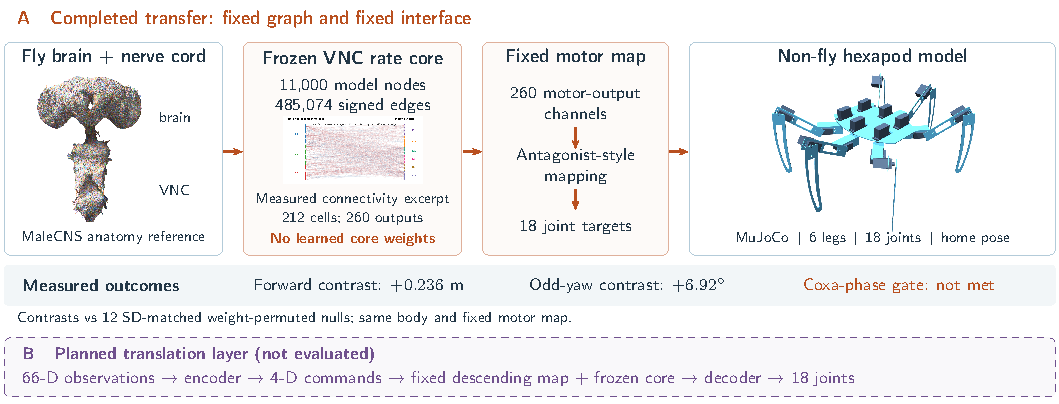
\includegraphics[width=0.96\textwidth]{overview_pipeline.pdf}
\caption{Completed transfer and planned translation layer. MaleCNS brain/VNC anatomy: Janelia FlyEM and collaborators, CC-BY~\cite{malecns}; the VNC is pivoted for visibility. This anatomy reference is broader than the selected modeled graph. The connectivity inset uses measured edges. The hexapod is rendered from the actual MuJoCo model in its home pose, not a walking result. Solid arrows show the fixed transfer; the dashed strip is proposed and untested. The earlier 49-dimensional pilot was inconclusive.}
\label{fig:overview}
\end{figure*}

\section{Biological Reference and Related Work}
\label{sec:related}
MaleCNS files are publicly available neural data~\cite{malecns}; this computational study used no new human or animal subjects, and all body results came from simulation. The dataset contains sensory, intrinsic, descending, ascending, and motor populations; the biological VNC receives brain commands and body feedback before producing muscle-related output~\cite{takemura2024manc,cheong2026premotor}. Our completed branch models only the selected VNC graph with externally injected current into model nodes corresponding to DNg100/DNb08. It does not simulate every sensory path, and it evaluates output after a declared coordinate conversion.

A graph can behave differently when its outputs drive a different body. Reservoir frameworks use recurrent dynamics as a computational substrate and learn a separate readout~\cite{damicelli2022reservoir,suarez2024conn2res}. A robot driven by a connectome can show actions that depend on sensor placement, actuator mapping, and body mechanics~\cite{valencia2023robot}. We therefore freeze the selected VNC graph and motor map and measure phase independently of displacement.

We also compare the MaleCNS data against explicit null models. Network analyses of \textit{Drosophila} compare empirical wiring against a female whole-brain connectome and random graphs that preserve different properties, including degree and mesoscale structure~\cite{lin2024network}. Our weight-permuted nulls preserve topology and permute the signed weight multiset. Rewired nulls change topology through directed edge swaps while preserving row degree, column degree, and the same signed weight multiset. Spatial distance, neuropil blocks, and all cell-type roles remain unconstrained. Accordingly, our comparison supports only a graph-dependent contrast relative to these specified nulls, not a universal claim about anatomical organization.

\section{Methods}
\label{sec:methods}
\subsection{MaleCNS-v1.0-Derived VNC Graph Construction}
We used the official MaleCNS v1.0 full-CNS annotation and connectivity files to build an all-leg, VNC-centered closure with all premotor candidates in scope; DNg100/DNb08 input nodes received fixed descending-neuron drive~\cite{malecns,takemura2024manc}. The closure contains 11,000 model nodes (1,325 descending inputs; six DNg100/DNb08 input nodes) and retains traced motor, premotor/descending predecessor, rhythm-core, and upstream cells. The fixed candidate rule required a trace, VNC-intrinsic annotation, one of 66 published coordination labels, and neuromere T1, T2, or T3~\cite{cheong2026premotor}. It yielded 212 selected cells and 62 of 66 labels; four labels were absent or outside scope. The 212 cells are candidates within the 11,000-node closure; the fixed map later sends 260 motor outputs to 18 joints. After an absolute synapse floor of five, the graph contains 485,074 signed nonzero edges.

Each retained edge carries a connectome-derived signed weight. Raw edge magnitude is the integer synapse count from the release; we apply only the neurotransmitter sign and the floor of five, with no additional weight normalization. Acetylcholine edges were positive; gamma-aminobutyric acid (GABA) and glutamate edges were negative; we omitted unclassified or modulatory signs. This sign is a model convention; it has no validated physiological synaptic-efficacy interpretation. The graph stores postsynaptic rows and presynaptic columns. We also retained a T1-only graph with 4,418 nodes and 144,214 signed edges for rhythm characterization.

\subsection{Frozen Rate Model}
The selected VNC state $v$ follows a bounded recurrent rate model. At each substep, the network computes
\begin{equation}
  \begin{aligned}
  v_{t+1}&=(1-\Delta t/\tau)v_t\\
  &\quad+\frac{\Delta t}{\tau}\max\left(0,c\tanh\left[
  \frac{a}{c}(g_W Wv_t+I-\theta)\right]\right),
  \end{aligned}
\label{eq:vnc}
\end{equation}
where $W$ is the frozen signed graph, $I$ is the fixed descending current, $c$ is the firing-rate cap, $a$ is activation gain, and $\theta$ is threshold. We used $\tau=0.02$ s, $\Delta t=0.005$ s, four substeps per control sample, $g_W=0.03$, and bilateral drive of 100 into the six DNg100/DNb08 inputs. We used $\theta=7.5$, $a=1$, and $c=200$. One heterogeneity draw used NumPy seed 1 and independent normal draws with standard deviations $(0.002,0.1,0.6,10)$ for $(\tau,a,\theta,c)$; values were lower-clipped at $(\Delta t,10^{-3},0,1)$ and remained unchanged across conditions.

\subsection{Motor Map and Hexapod Body}
The output vector contains signed motor-pool activity for six legs and five fly joint groups. A fixed label rule assigns flexor/extensor-style motor-pool polarity, and the map computes flexor-minus-extensor activity for each pool. It maps fly coxa to hexapod coxa, averages trochanter/femur activity for hexapod femur, and averages available tibia/tarsus activity for hexapod tibia; missing pools stay at home stance. The three map gains are $(-0.55,0.65,0.65)$.

The target angles drive an 18-joint PhantomX-style hexapod in MuJoCo, a physics simulator~\cite{todorov2012mujoco}. We use the project hexapod XML asset with MuJoCo 3.12.0 and its 0.002 s simulation step; each 50 Hz control sample advances 10 physics steps. Each state sets body height to 0.15 m and the prescribed yaw, then settles joints for 0.7 s toward the MJCF home stance under 50 Hz proportional-derivative (PD) torque ($k_p=3.0$, $k_d=0.05$). The simulation passes targets directly in MuJoCo joint order and applies no post-map side/world sign transform. The same map and body serve the measured graph and every control graph. The map is a fixed engineering rule, not a fitted physiological readout. We included a hand-written tripod clock as a temporal-order control.

\subsection{Controls and Endpoints}
The primary control family uses 12 weight-permuted null seeds. Each null keeps the directed topology and permutes its signed weight multiset. The rewired null changes topology through directed edge swaps while preserving row degree, column degree, and the same signed weight multiset. For amplitude matching, we center each control history on its own channel mean and rescale it so all 18 joint-target channels match the measured graph's temporal standard deviation; temporal means and ordering remain control-specific. This matches only marginal channel scale, not cross-channel covariance, phase, target bounds, or delivered torque. The maximum standard-deviation error across channels is $3.61\times10^{-6}$ rad.

The primary graph-null endpoint was amplitude-matched forward displacement; the coxa-phase proxy was a prespecified neural diagnostic before the fixed motor map, without body-level footfall scoring. Odd yaw, body sensitivity, the 3 s study, and rewiring dose were secondary or diagnostic.

Rhythm used that heterogeneity draw, 1,500 samples at 0.02 s (30 s; first 15 s discarded), without smoothing. Tripod phase used coxa traces for A $=\{\mathrm{T1L,T2R,T3L}\}$ and B $=\{\mathrm{T1R,T2L,T3R}\}$. The 1.5--4 Hz analytic-signal test passed only when all six within-tripod pairs were within 0.15 cycles of zero and all nine cross-tripod pairs were within 0.15 cycles of half a cycle; we used no minimum phase-concentration criterion.

Forward and odd-yaw endpoints used 8 s rollouts. Body sensitivity used nine labeled runs from seven unique settings (six perturbations, one nominal run, and two nominal technical repeats); the equal-weight mean includes all nine labels, not nine independent settings. The 3 s study compared open-loop real VNC, brain-coupled VNC, column-permuted VNC, random descending drive, and a hand-written tripod clock. Null seeds ranged from 20260830 to 20260841; shared episode starts used seeds 20260829 to 20260848.

Graph-null contrasts used one measured graph, 20 shared starts, and 12 null seeds; odd yaw used 20 starts per direction. Graph, heterogeneity draw, body, map, and starts stayed fixed. Null seeds were independent only conditional on these components. Intervals and p-values describe sampled null-network variability, not uncertainty over graph construction, body, map, or starts.

We held the measured mean fixed and resampled null-seed means for conditional 95\% percentile-bootstrap intervals. The seed-level benchmark enumerates flips of 12 null differences under conditional independence and uniform sign symmetry; it is a sign-flip p-value, not a randomization test. Five-condition paired tests used exact two-sided sign flips under the same assumptions and are conditional diagnostics, not randomization tests. Ranges are 95\% percentile-bootstrap CIs with paired resampling. For provenance, 240 outcomes formed 12 seed summaries, so the primary contrast used seed-level summaries. Holm adjustment covered three predeclared 3 s path comparisons; no global adjustment spans endpoint families. Pearson coxa correlations and analytic gate counts came from separate analyses (all\_legs\_coordination.json and bodyfix\_vnc\_phase\_probe\_e0.json); phase results are pair counts from one fixed trace.

Path is cumulative planar step distance; forward displacement is final planar displacement projected onto post-settle yaw, and planar displacement is Euclidean endpoint distance. In the 3 s study, catch means prey distance $<0.25$ m and fall means minimum body height $<0.08$ m. Yaw uses wrapped angular differences; odd yaw is half the positive-minus-negative response.

We fixed graph and motor-map choices before evaluation. No result uses a learned VNC weight, learned motor-map parameter, reward term, or target trajectory to select the graph or motor map. The fixed body controller tracks predetermined joint targets during simulation, and performance never selects the graph.

The project files contain the analysis scripts and canonical JSON/CSV records named in this paper. These records retain graph hashes, run seeds, and bootstrap settings; the project README lists commands for rebuilding the graph and study summaries.

\section{Results}
\label{sec:results}
\subsection{VNC output and coxa-phase proxy}
The T1 graph produces a dominant motor-output peak at 2.467 Hz and an autocorrelation frequency of 2.500 Hz. In one fixed trace with 1,500 samples, the mean autocorrelation peak is 0.342, opposing motor pools correlate at $-0.321$, and left/right pools correlate at $+0.031$. These values show dynamic activity under constant descending drive. They do not by themselves establish six-leg coordination.

At the selected VNC motor-output layer, the coxa audit gives mean Pearson within-tripod correlations of $-0.057$ for tripod A and $+0.307$ for tripod B, with cross-tripod Pearson correlation $-0.185$ in one deterministic trace. The analytic-signal phase gate accepts 3 of 6 within-tripod pairs and 3 of 9 cross-tripod pairs. The trace therefore does not pass the prespecified neural coxa-phase proxy. The fixed map transmits all 18 target channels, and body joint angles track those targets with mean Pearson correlation 0.438.

\subsection{Matched Graph-Null Contrast in Forward Displacement}
Under per-channel marginal temporal-SD matching, the measured graph produces 0.224 m mean forward displacement across 20 episodes. The 12 weight-permuted null seeds are each summarized over the same starts and average $-0.012$ m, giving a measured-minus-null difference of $+0.236$ m with a conditional 95\% null-seed interval of [$+0.187,+0.281$] m. All 12 sampled null-network means fall below the measured-graph mean. A conditional one-sided sign-flip benchmark under conditional independent, uniform sign symmetry gives $p=0.000244$; we treat it as a sign-flip p-value, not a randomization p-value. This result matches marginal temporal scale at all 18 joint targets, but not cross-channel covariance, phase, or delivered torque.

The same direction appears in the shorter paired control study. Across 20 shared 3 s starts, real open-loop VNC path is 0.351 m [0.348, 0.353], while column-permuted VNC path is 0.084 m [0.080, 0.090]. Their paired difference is $+0.266$ m [0.261, 0.271], exact two-sided paired sign-flip $p=1.91\times10^{-6}$ and Holm-adjusted $p=5.72\times10^{-6}$. The brain-coupled VNC path is 0.286 m [0.224, 0.340], compared with 0.348 m [0.317, 0.378] for random descending drive. Their paired difference is $-0.062$ m [$-0.119,-0.009$]. The exact two-sided paired sign-flip test gives Holm-adjusted $p=0.042$.

Against the hand-written tripod clock, real open-loop path is higher by 0.171 m [0.119, 0.223], exact two-sided paired sign-flip $p=5.72\times10^{-6}$ and Holm-adjusted $p=1.14\times10^{-5}$. Mean motor temporal SDs were 0.140 and 0.067 in model-rate units for real open-loop and column-permuted VNC, respectively, so we did not amplitude-match this comparison. Zero of 20 episodes in each of five fixed conditions met the union event (catch or fall); each condition-specific Wilson 95\% upper bound is 0.161 (16.1\%). The hand-written tripod clock stayed upright in this setup. This open-loop temporal-order diagnostic is separate from a network-wiring null; prey pursuit and gait transfer remain untested.

\subsection{Yaw contrast and sensitivity in one body}
An asymmetric bilateral descending drive produces a measured odd-yaw response of 7.441$^{\circ}$ across 20 shared starts per turn direction. We define odd yaw as half the difference between the $+0.5$ and $-0.5$ drive yaw changes. Relative to same-turn amplitude-matched weight-permuted nulls, the difference is $+6.916^{\circ}$ [4.892, 8.899] with a conditional 95\% null-seed interval; all 12 sampled controls are below the measured graph. An exact one-sided conditional sign-flip test gives $p=0.000244$ under sign symmetry. This is an odd-yaw contrast under the fixed map. A separate constant-drive VNC trace does not pass the neural coxa-phase proxy, so task-level steering remains unestablished.

Across nine labeled runs of one configured body (20 episodes per setting; 12 null seeds), the forward difference stays positive. The equal-weight margin is 0.235 m [$+0.187,+0.276$] m and the worst-case contrast is 0.242 m [$+0.191,+0.286$] m (conditional 95\% null-seed intervals). The latter is the minimum measured displacement minus the mean of the corresponding null-seed minima. All 12 sampled null summaries fall below the measured minimum. Six runs perturb body parameters; three labels share one nominal setting and are not independent body settings. This is parameter sensitivity within one morphology, not body generalization. Figure~\ref{fig:robustness} shows the body perturbations and rewiring-dose probe; the measured points remain above the matched nulls across the six perturbations.

\begin{figure*}[t]
\centering
\includegraphics[width=0.96\textwidth]{robustness_rewiring.pdf}
\caption{Secondary graph and body analyses. (A) Measured-graph forward displacement exceeds per-channel SD-matched, weight-permuted nulls at six non-default body settings; three nominal labels share one body. Blue points: measured means; orange squares/ranges: null means and central 95\% seed ranges over 12 nulls. (B) Degree-preserving rewiring gives descriptive Spearman $\rho=-0.829$ across six aggregate means; $\alpha$ equals accepted swaps divided by half the edge count. Shading shows conditional 95\% bootstrap intervals over 12 rewired seeds; each setting uses 20 shared starts.}
\label{fig:robustness}
\end{figure*}

\subsection{Forward displacement changes across rewiring doses}
Degree-preserving rewiring provides a dose-based structural probe. Across 20 measured-graph baseline episodes and 12 rewired seeds summarized over 20 starts at each nonzero dose, mean forward displacement falls from 0.224 m at zero rewiring to $-0.009$ m at the maximum tested dose $\alpha=1$. The parameter $\alpha$ equals accepted swaps divided by half the edge count; $\alpha=1$ is the maximum tested dose, not complete randomization. The six aggregate means give a descriptive Spearman $\rho=-0.829$; the intermediate curve is nonmonotone. The maximum-dose loss relative to the measured graph is 0.233 m [0.210, 0.254] with a conditional 95\% null-seed interval. At $\alpha=0.1$, 25/240 episodes fell (10.4\%); 17 falls came from one rewired seed and 8 from another. Because episodes share rewired seeds, we treat this rate as descriptive and omit an episode-level interval. Rollouts continued after the threshold, so forward displacement includes post-fall motion. The dose series is exploratory and supplies no trend test.

\section{Discussion}
\label{sec:discussion}
The selected VNC graph produces time-varying output and, relative to the specified controls, more forward displacement and larger odd yaw. Its output does not pass the neural coxa-phase proxy, and we ran no separate body-level footfall-phase gate. Thus body mechanics might transform the signal into an alternating tripod, but transferred gait remains unestablished. The measured result supports only graph-dependent motor drive under the tested nulls.

Several controls narrow interpretation. The 212-cell inventory follows the fixed MaleCNS selection rule. Per-channel marginal-SD matching controls temporal scale at joint targets, but not covariance, phase, or torque. Rewiring probes the tested edge-swap procedure, not a unique mechanism. Weight-permuted and rewired nulls preserve different degree and weight properties; neuropil blocks, distances, motifs, and cell-type roles remain unconstrained~\cite{lin2024network}.

The cross-body setup also limits biological interpretation. The MaleCNS-v1.0-derived VNC graph models a fly nerve cord, while PhantomX differs in geometry, joints, torque limits, mass, and ground interactions. The map averages five fly joint groups into three robot joints per leg; all 260 channels feed the fixed map, but SD matching uses only its 18 joint targets. One body supports parameter sensitivity within one morphology, not morphology generalization.

The model omits biological delays, muscle mechanics, and sensory dynamics. Constant drive limits the coxa result, and the separate 3 s study found lower brain-coupled path than random-drive path.

\subsection{Translation layer remains untested}
Completed experiments freeze the selected VNC graph and motor map. The planned
66-dimensional layer would learn walking and balance while the selected VNC graph
and motor map remain fixed. It
would encode body state, target direction, joint state, and previous action into
four commands (go, steer, family, and walkdn); walkdn targets DNg100/DNb08. A
fixed $4\times1325$ map would drive the core, and a trainable decoder would output
18 joint targets. The encoder, decoder, and Proximal Policy Optimization (PPO)
value critic would train. Target direction would bypass fly sensory input.

A separate four-latent 49-dimensional joint-position/joint-velocity (qpos/qvel)
PPO pilot ran 4,999,936 steps
per arm; its measured-graph arm fell in 12/12 evaluation episodes, so the record
is inconclusive. A v3 attempt used the same interface, completed Stage 1, and
ended before valid preregistered three-arm evaluation; partial trajectories were
excluded. Neither attempt evaluated the proposed 66-dimensional design; we report
no walking, balance, or target-reaching result.

\section{Conclusion}
\label{sec:conclusion}
The measured MaleCNS-v1.0-derived VNC graph produced higher matched forward displacement and odd-yaw response than specified nulls. The contrast persisted across six parameter perturbations. Three nominal labels share one body, and the coxa trace did not pass the neural coxa-phase proxy. This supports graph-dependent motor drive through the tested interface; gait organization and the proposed walking/balance layer remain unvalidated.

\bibliographystyle{IEEEtran}
\bibliography{flycraft_bibm_draft}

\end{document}
